\chapter{Introduction}

\section{Proteins and Protein Folding}

\subsection{Protein Structure Prediction - Motivation}
    
% \begin{itemize}
%     \item Primary $\to$ Tertiary (\href{https://www.youtube.com/watch?v=W9J294X4FbY}{https://www.youtube.com/watch?v=W9J294X4FbY})
%     \item Neural Networks for the problem
%     \item CASP and history of protein folding
%     \item How good are the current approaches?
%     \item difficulties and short overview of current approaches
% \end{itemize}
    
Proteins are one of the essential cellular macromolecules. 
They perform several functions as receptors, enzymes, antibodies as well as being the structural components of the cell.
% The basic building blocks of proteins are amino-acids.
In nature, most proteins consist of only 20 proteogenic amino acids linked together by peptide bonds.
The peptide bonds form a linearly connected chain of amino-acids also called the primary structure of the protein.
This primary structure can be represented in the simple file format, such as FASTA, using single letters to represent particular amino acids.
The 1-letter codes with their corresponding amino acids are shown in the Table \ref{tab:aa_codes}.

\begin{table}[]
    \centering
    \begin{tabular}{r|c|r|c|}
        Alanine & A & Arginine & R \\
        Asparagine & N & Aspartic acid & D \\
        Cysteine & C & Glutamine & Q \\
        Glutamic acid & E & Glycine & G \\
        Histidine & H & Isoleucine & I \\
        Leucine & L & Lysine & K \\
        Methionine & M & Phenylalanine & F \\
        Proline & P & Serine & S \\
        Threonine & T & Tryptophan & W \\
        Tyrosine & Y & Valine & V
    \end{tabular}
    \caption{Standard amino acid abbreviations}
    \label{tab:aa_codes}
\end{table}

% add something about secondary structure?

In their native state, the proteins fold into a stable three dimensional structures which allows them to perform various tasks.
% because of other forces such as hydrophobicity... 
This three dimensional structure is also called the tertiary structure of the protein.
The very delicate conformation of the protein is crucial for the correct functioning of the cell.
In rare cases, when the structure is corrupted, it might result in serious diseases such as cystic fibrosis, Parkinson's disease, Huntington's disease, cancer and many others \cite{protein_misfolding_diseases}.

It is hypothesized that the instructions for the folding are encoded in the primary protein structure. 
% what is a denatured protein?
The thermodynamic theory states, that if a denatured protein occurs in an environment it was selected for (pH, ionic strength, etc.) then it will fold into a state with minimum Gibbs free energy.
% should this be mentioned before, since we already used the term native state?
This state is also called a "native state" of a protein. 
Christian B. Anfinsen and his group published a famous paper in 1973, where they managed to denature ("unfold") a protein (bovine pancreatic ribonuclease) with urea - shown in Figure \ref{fig:primarytertiary}a). 
Afterwards, when they removed urea the protein folded back into the same state as the initial one \cite{anfinsen}.
% 2 types of denaturation?
    
\begin{figure}[b!]
    \centering
    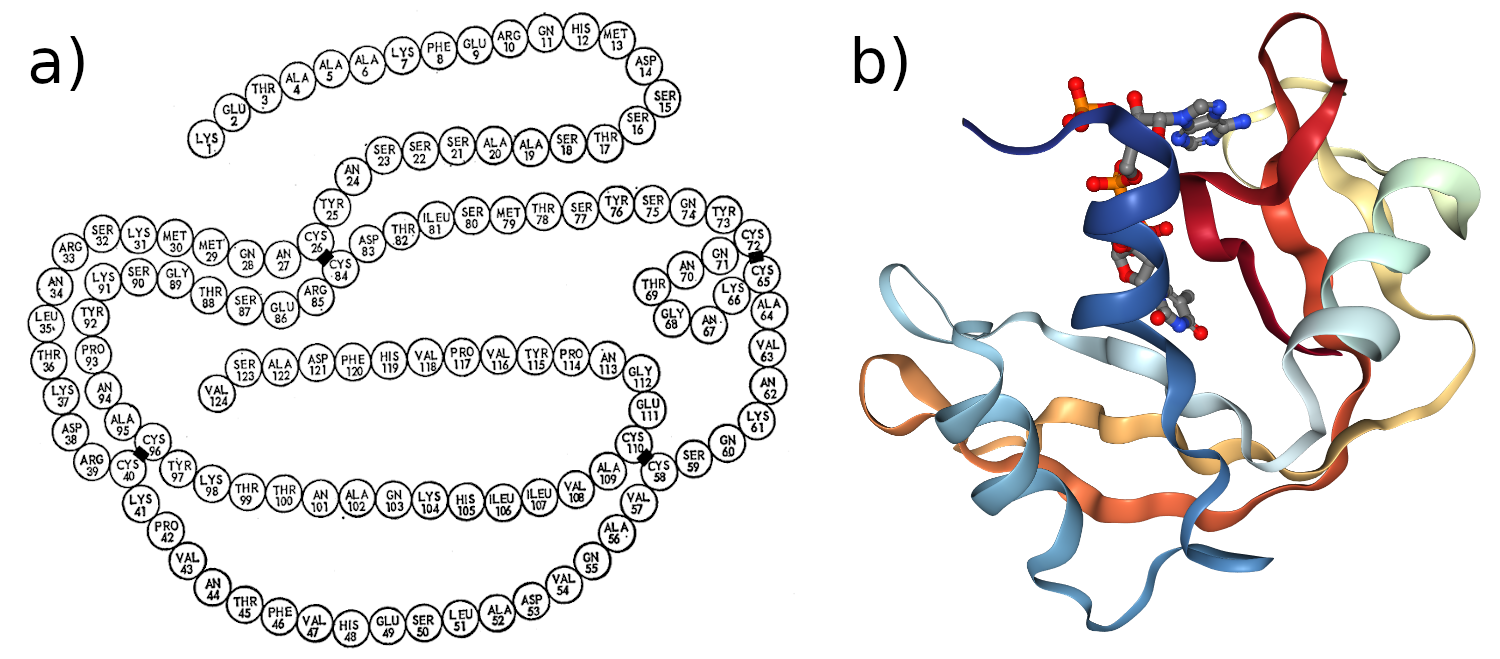
\includegraphics[scale = 0.25]{imgs_tomas/primary_tertiary.png}
    \caption{Primary (a)) \cite{anfinsen} and tertiary structure (b)) \cite{pdb} of bovine pancreatic ribonuclease.}
    \label{fig:primarytertiary}
\end{figure}
    
This suggests a link between the primary and tertiary structure of a protein which has not been uncovered, and likely never will be. % why it will never be? 
% ...and because of its complexity, likely never will be.
    
To get an idea of how complex the problem is, lets consider a simple scenario. 
Lets say, that we have protein of length 100 and each amino acid residue consists of two rotable bonds. 
If there were only 2 allowed angles (cf. Ramachandran plot in later section) per rotable bond, then the total number of possible conformations is $(2\cdot2)^{100} = 4^{100}$. 
Let say that we have a computer that can generate one of these unique conformations, compute its Gibbs energy and check whether it is smaller than the current minimum. 
If this could be done in a picosecond ($10-{12} s$), than to find the optimal structure would take roughly $5 \cdot 10^{43}$ years (universe is $\sim 13.8\cdot10^9$ years old).
    
Experimental approaches of obtaining the spatial structure include X-ray crystallography and Nuclear Magnetic Resonance (NMR) with the former being responsible for majority of known structures. 
Since the relative distances between amino acids are in order of \AA ngstroms ($\sim10^{-10}$m), visible light ($\sim10^{-7}$m) can not be used to observe the structures. 
Hence the higher energy X-rays which operate within this region. 
One major disadvantage of experimental techniques is their cost and that they are time consuming.
The ability to determine tertiary structure of a protein with decent accuracy would help especially in medicine and research, by designing new ones to battle with diseases.
% (???WHAT ACCURACY IS DECENT???)
    
Luckily in this age we have an access to large amount of known structures and many more known primary structures. 
Given this and the fact of the rapid rise of machine learning frameworks we can look at the problem from different perspective.
    
Given a large set of primary structures of proteins from different species, we should be able to construct clusters of proteins belonging to the same family. 
These proteins are likely performing similar functions in different species and should have similar tertiary structures. 
Given a random amino acid sequence we should be able to find similar sequences and construct the Multiple Sequence Alignment - MSA. 
In the MSA we should observe linked sites - sites where the correlation of amino acids is far from random. 
Non random site linkage might be a result of selective pressure (region of protein responsible for a certain function), a direct contact between two non-convalently linked amino acids or indirect/mediated contact between two amino acids. 
Thus we believe that the MSA holds information about the spatial proximity of amino acid pairs and is the main assumption of our thesis report. 
We can use this MSA-induced data and predict the inter-residue distances which we can further use for the generation of the full tertiary structure.
    
\subsection{Amino acids - Basic building blocks, and their characteristics}
    
% \begin{itemize}
%     \item Properties of Amino Acids, Bonds (Peptidic, Hydrogen, ...)
%     \item Distance between AA, torsion angles
%     \item Primary/Secondary/Tertiary/Quaternary structure
%     \item domains
        
% \end{itemize}
    
% \begin{itemize}
%     \item What are proteins? What is their structure? Why is it important to know their 3D structure?
%     \item Primary/Secondary/Tertiary/Quaternary structure
%     \item What is protein folding, its history and why the knowledge of secondary structure is not important for predicting tertiary structure?
% \end{itemize}

% \section{Protein Structure Prediction}
% \begin{itemize}
%     \item difficulties and short overview of current approaches
%     \item How good are the current approaches?
%     \item What is CASP and what happened in 2018
% \end{itemize}
